






%%%%%%%%%%%%%%%%%%%%%%%%%%%%%%%%%%%%%%%%%%%%%%%%%%%%%%%%%%%%%%%%%
% Apresentação sobre K-Nearest Neighbors (KNN)
% Gerado por Gemini
% Baseado em pesquisa aprofundada sobre o algoritmo
%%%%%%%%%%%%%%%%%%%%%%%%%%%%%%%%%%%%%%%%%%%%%%%%%%%%%%%%%%%%%%%%%

\documentclass{beamer}

% --- PACOTES ---
\usepackage[utf8]{inputenc} % Codificação de entrada
\usepackage[T1]{fontenc}      % Codificação da fonte
\usepackage{lmodern}          % Fonte Latin Modern
\usepackage[brazil]{babel}    % Idioma
\usepackage{amsmath}          % Fórmulas matemáticas avançadas
\usepackage{graphicx}         % Inclusão de imagens
\usepackage{xcolor}           % Cores
 \usepackage{booktabs} 
 \usepackage{array} 
\usepackage[backend=biber]{biblatex} % Gerenciamento de bibliografia
% --- CONFIGURAÇÕES DO TEMA ---
\usetheme{Madrid}
\usecolortheme{default}

% --- INFORMAÇÕES DO TÍTULO ---
\title[Análise de Algoritmos de ML]{Análise  de K-Means e KNN: Fundamentos e Aplicações Práticas}
\subtitle{Explorando Geometria, Escalabilidade e Impacto Prático em Machine Learning}
\author[Bruno M.M. Vieira]{Bruno Martins Mendes Vieira}
\institute[PPGFA]{Programa de Pós-Graduação em Física Ambiental}
\date{27 de Agosto de 2025}
\AtBeginSection[]{
  \begin{frame}<beamer>
    \frametitle{Roteiro da Apresentação}
    \tableofcontents[currentsection,currentsubsection]
  \end{frame}
}
\begin{document}

% --- SLIDE DE TÍTULO ---
\begin{frame}
  \titlepage
\end{frame}

% --- SLIDE DE ROTEIRO ---
\begin{frame}
  \frametitle{Roteiro da Apresentação}
  \tableofcontents
\end{frame}
%%%%%%%%%%%%%%%%%%%%%%%%%%%%%%%%%%%%%%%
\section{KNN}
\subsection{Contexto Histórico do KNN}
\begin{frame}{Introdução ao Contexto Histórico do KNN}
\begin{itemize}
\item<1-> O algoritmo K-Nearest Neighbors (KNN) é um dos métodos mais intuitivos e fundamentais em aprendizado de máquina.
\item<2-> Sua história pode ser dividida em três fases principais:
\begin{itemize}
\item Origem (1951)
\item Formalização e Popularização (1967)
\item Evolução e Otimização (1970 em diante)
\end{itemize}
\end{itemize}
\end{frame}

% Slide 2: A Origem (1951)
\begin{frame}
\frametitle{A Origem do KNN: Um Projeto Militar Secreto (1951)}
\begin{itemize}
\item<1-> \textbf{Contexto:} Surgiu em um contexto militar, logo após a Segunda Guerra Mundial\@, diferente de algoritmos acadêmicos tradicionais.
\pause
\item \textbf{Quem:} Formulado por \textbf{Evelyn Fix} e \textbf{Joseph Hodges}, estatísticos da Força Aérea dos EUA.
\item \textbf{Onde:} Desenvolvido na \textbf{Escola de Medicina da Aviação da Força Aérea dos EUA}.
\item \textbf{O que:} Relatório técnico de 1951, \textit{``Discriminatory Analysis, Nonparametric Discrimination: Consistency Properties''}.
\begin{itemize}
\item Propôs um método de classificação não-paramétrico para classificar objetos (ex.: aeronaves amigas ou inimigas) sem suposições sobre a distribuição dos dados.
\end{itemize}
\pause
\item \textbf{Curiosidade:} O trabalho não foi publicado abertamente na época, provavelmente por ser confidencial, permanecendo restrito por mais de uma década.
\end{itemize}
\end{frame}

% Slide 3: Formalização e Popularização (1967)
\begin{frame}
\frametitle{Formalização e Popularização (1967)}
\begin{itemize}
\item<1-> \textbf{Contexto:} O KNN ganhou notoriedade nos anos 60, entrando no campo acadêmico da ciência da computação e teoria da informação.
\item<2-> \textbf{Quem:} \textbf{Thomas Cover} e \textbf{Peter Hart}, da Universidade de Stanford.
\item<3-> \textbf{O que:} Publicaram o artigo \textit{``Nearest Neighbor Pattern Classification''} em 1967, que foi crucial por:
\begin{itemize}
\item<4-> Formalizar a regra do vizinho mais próximo (\(k=1\)).
\item<5-> Provar que a taxa de erro do KNN não é pior que o dobro da taxa de erro do classificador de Bayes.
\item<6-> Popularizar o termo \textbf{``Nearest Neighbor''} na comunidade de reconhecimento de padrões e aprendizado de máquina.
\end{itemize}
\end{itemize}
\end{frame}

% Slide 4: Evolução e Otimização (1970 em diante)
\begin{frame}
\frametitle{Evolução e Otimização (1970 em diante)}
\begin{itemize}
\item<1-> \textbf{Contexto:} Após 1967, o KNN tornou-se um algoritmo fundamental, ensinado em cursos de aprendizado de máquina.
\item<2-> \textbf{Avanços:}
\begin{itemize}
\item<3-> \textbf{KNN Ponderado:} Introdução de pesos para vizinhos mais próximos.
\item<4-> \textbf{Estruturas de dados:} Desenvolvimento de \textit{k-d trees} para buscas mais rápidas em grandes conjuntos de dados.
\item<5-> \textbf{Fuzzy KNN:} Em 1985, James Keller introduziu uma versão que lida com incertezas na classificação.
\end{itemize}
\end{itemize}
\end{frame}

% Slide 5: Conclusão
\begin{frame}
\frametitle{Conclusão}
\begin{itemize}
\item O KNN nasceu como uma solução prática para um problema militar.
\item Após um período de obscuridade, foi formalizado e popularizado pela academia.
\item Tornou-se um dos algoritmos mais intuitivos e duradouros do aprendizado de máquina.
\item Sua simplicidade e flexibilidade continuam a inspirar avanços e aplicações.
\end{itemize}
\end{frame}
%%%%%%%%%%%%%%%%%%%%%%%%%%%%%%%%%%%%%%%%%%%%%%%%%%%%%%%%%%%%%%%%%
\subsection{Introdução ao Algoritmo KNN}
%%%%%%%%%%%%%%%%%%%%%%%%%%%%%%%%%%%%%%%%%%%%%%%%%%%%%%%%%%%%%%%%%

\begin{frame}{O Que é o K-Nearest Neighbors (KNN)?}
    \begin{itemize}
        \item \textbf{Algoritmo Supervisionado:} Usado para classificação e regressão.
        \item \textbf{Baseado em Instâncias:} Não ``aprende'' um modelo explícito a partir dos dados de treino. Ele memoriza todo o conjunto de treinamento.
        \item \textbf{Aprendizagem Preguiçosa (Lazy Learning):} Todo o cômputo ocorre no momento da predição, não durante o ``treinamento''.
        \item \textbf{Premissa Central:} Pontos de dados semelhantes existem em proximidade uns dos outros. A ``semelhança'' é medida por uma métrica de distância.
    \end{itemize}
\end{frame}

%\begin{frame}
    %\frametitle{Como o KNN Funciona? (Classificação)}
    %\begin{enumerate}
     %   \item \textbf{Escolha de K:} Definir o número de vizinhos (K) a serem considerados.
    %    \item \textbf{Cálculo de Distâncias:} Para um novo ponto de dado, calcular a distância para todos os pontos no conjunto de treinamento.
   %     \item \textbf{Identificar Vizinhos:} Selecionar os K pontos de treinamento mais próximos (os "vizinhos").
  %      \item \textbf{Votação Majoritária:} Atribuir ao novo ponto a classe mais comum entre os K vizinhos.
 %   \end{enumerate}
%\end{frame}
\subsection{Funcionamento}
\begin{frame}{Como o KNN Funciona? (Classificação)}
    \begin{figure}
        \centering
        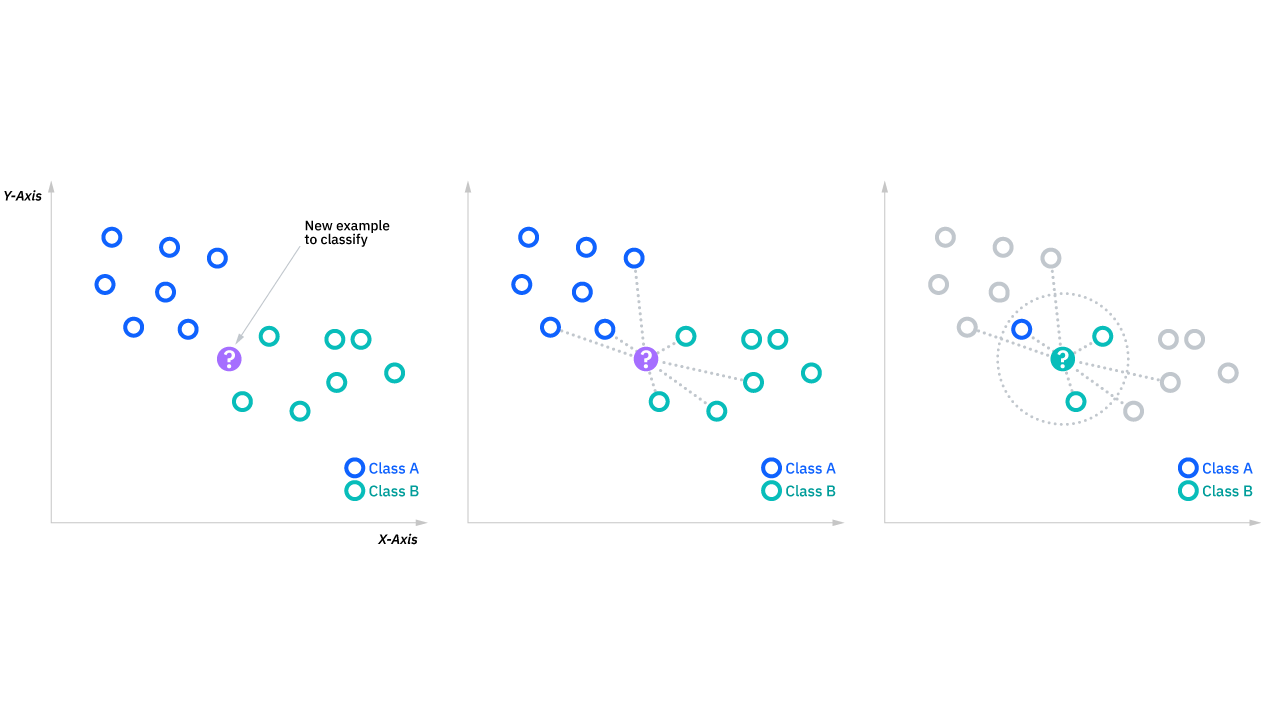
\includegraphics[width=0.8\linewidth]{imagens/KNN.png}
        \caption{Diagrama do funcionamento do KNN \cite{ibm_knn_br}}
    \label{fig:diagramaknn}
    \end{figure}
\end{frame}
%%%%%%%%%%%%%%%%%%%%%%%%%%%%%%%%%%%%%%%%%%%%%%%%%%%%%%%%%%%%%%%%%
\subsection{A Geometria das Métricas de Distância}
%%%%%%%%%%%%%%%%%%%%%%%%%%%%%%%%%%%%%%%%%%%%%%%%%%%%%%%%%%%%%%%%%

\begin{frame}{A Escolha Crítica: A Métrica de Distância}
    A forma como medimos a ``proximidade'' define a fronteira de decisão do modelo. A escolha da métrica depende da natureza dos dados.


\end{frame}

\begin{frame}{Distância Euclideana {($L_2$)}}
    É a distância mais intuitiva: o comprimento de uma linha reta entre dois pontos.
    \begin{equation}
        d(p, q) = \sqrt{\sum_{i=1}^{n} (p_i - q_i)^2}
    \end{equation}
\pause
\textbf{Exemplo:}
\begin{itemize}
    \item Pontos: $p = (2, 3)$, $q = (5, 7)$
\end{itemize}
\pause
\begin{align*}
    d(p, q) &= \sqrt{(2 - 5)^2 + (3 - 7)^2}\\
    &= \sqrt{(-3)^2 + (-4)^2}\\ &= \sqrt{9 + 16}\\ &= \sqrt{25} \\&= 5
\end{align*}


\end{frame}
\begin{frame}{Dimensionalidade}
\centering
    Mas, e quando aumentamos para 4 dimensões?
\end{frame}
\begin{frame}{Clientes com quatro características}
    
\begin{itemize}
    \item \textbf{Idade}
    \item \textbf{Nº de Compras}
    \item \textbf{Avaliação Média} 
    \item \textbf{Tempo como Cliente} 
\end{itemize}

Perfil de Cliente:
\begin{itemize}
    \item \textbf{Cliente A}: (Idade: 30, Compras: 15, Avaliação: 4, Tempo: 24)
    \item \textbf{Cliente B}: (Idade: 35, Compras: 10, Avaliação: 5, Tempo: 36)
\end{itemize}


\end{frame}
\begin{frame}{Distância de Manhattan ($L_1$)}
    Também conhecida como ``distância do táxi''.
     \[d(p, q) = \sum_{i=1}^{n} |p_i - q_i|\]
    
    \begin{itemize}
        \item \textbf{Intuição Geométrica:} Distância percorrida em uma grade (como quarteirões de uma cidade).
        \item \textbf{Uso Comum:} Eficaz em espaços de alta dimensão.
    \end{itemize}
\end{frame}



% Slide 2: Manhattan Distance Calculation
\begin{frame}{Distância Manhattan}


% Calculating for each dimension

\begin{itemize}
    \item \textbf{Idade}: $|35 - 30| = 5$
    \item \textbf{Nº de Compras}: $|10 - 15| = |-5| = 5$
    \item \textbf{Avaliação Média}: $|5 - 4| = 1$
    \item \textbf{Tempo como Cliente}: $|36 - 24| = 12$
\end{itemize}

% Summing the differences
\begin{equation}
d_{\text{manhattan}} = 5 + 5 + 1 + 12 = 23
\end{equation}

\textbf{Resultado}: A distância  Manhattan é \textbf{23}.
\end{frame}

% Slide 3: Euclidean Distance Calculation
\begin{frame}{Distância Euclideana}
\pause

% Calculating for each dimension

\begin{itemize}
    \item \textbf{Idade}: ${(35 - 30)}^2 = 5^2 = 25$
    \item \textbf{Nº de Compras}: ${(10 - 15)}^2 = {(-5)}^2 = 25$
    \item \textbf{Avaliação Média}: ${(5 - 4)}^2 = 1^2 = 1$
    \item \textbf{Tempo como Cliente}: ${(36 - 24)}^2 = 12^2 = 144$
\end{itemize}
\pause
% Summing and taking the square root
\begin{equation}
d_{\text{euclidiana}} = \sqrt{25 + 25 + 1 + 144} = \sqrt{195} \approx 13.96
\end{equation}

\end{frame}

% Slide 4: Comparison and Analysis
\begin{frame}{Comparação e Análise}
% Summarizing the results
\textbf{Distância:}
\begin{itemize}
    \item \textbf{Manhattan}: 23
    \item \textbf{Euclideana}: $\approx 13.96$
\end{itemize}

% Highlighting the impact of Dimension 4
\textbf{Ponto chave: Tempo como cliente}
\begin{itemize}
    \item \textbf{Manhattan}: Contribui com 12 de 23.
    \item \textbf{Euclideana}: Contribui $12^2 = 144$ em 195 (mais de  73\%).
\end{itemize}

% Explaining the difference
%\textbf{Insight}: A distância euclidiana é mais sensível a grandes diferenças em uma única dimensão, pois elas são elevadas ao quadrado. A distância de Manhattan proporciona uma contribuição mais equilibrada entre todas as dimensões, especialmente quando a maioria das diferenças é pequena.

\end{frame}



%%%%%%%%%%%%%%%%%%%%%%%%%%%%%%%%%%%%%%%%%%%%%%%%%%%%%%%%%%%%%%%%%
\subsection{Problemas e Variações}
%%%%%%%%%%%%%%%%%%%%%%%%%%%%%%%%%%%%%%%%%%%%%%%%%%%%%%%%%%%%%%%%%

\begin{frame}{A Maldição da Dimensionalidade}

    \begin{itemize}

        \item \textbf{Concentração de Distância:} Em alta dimensão, a distância entre o vizinho mais próximo e o mais distante de um ponto se torna quase a mesma.
    \end{itemize}
    \vspace{0.5cm}
    \textbf{Impacto no KNN:} A premissa de ``vizinho próximo'' perde o sentido, e a votação dos vizinhos se torna aleatória.
\end{frame}



\begin{frame}{O Trade-off Viés-Variância na Escolha de K}


\begin{table}[ht]
\centering
\label{tab:comparacaok}
\begin{tabular}{|>{\raggedright\arraybackslash}p{0.45\textwidth}|>{\raggedright\arraybackslash}p{0.45\textwidth}|}
\hline
\textbf{K Pequeno (e.g., K=1)} & \textbf{K Grande (e.g., K=N)} \\
\hline

\textbf{Alta Variância}: Sensível a ruídos e outliers. & \textbf{Baixa Variância}: Ignora nuances locais. \\
\hline
\textbf{Resultado}: \textit{Overfitting} (superajuste). & \textbf{Resultado}: \textit{Underfitting} (subajuste). \\
\hline
\end{tabular}
\caption{Comparação entre K Pequeno e K Grande}

\end{table}
\end{frame}



\begin{frame}{Variações: O KNN Ponderado}
    %Na versão padrão, todos os K vizinhos têm o mesmo peso.

    \begin{block}{A Ideia da Ponderação}
        Dar mais peso aos vizinhos mais próximos, usando o \textbf{inverso da distância} como peso.
    \end{block}
    
    \textbf{Vantagem:} Torna o modelo mais robusto a outliers e menos sensível à escolha exata de K.
\end{frame}

%%%%%%%%%%%%%%%%%%%%%%%%%%%%%%%%%%%%%%%%%%%%%%%%%%%%%%%%%%%%%%%%%
%%%%%%%%%%%%%%%%%%%%%%%%%%%%%%%%%%%%%%%%%%%%%%%%%%%%%%%%%%%%%%%%%

\begin{frame}
    \frametitle{A Vantagem do ``Lazy Learning''}
    \begin{itemize}
        \item \textbf{Sem Custo de Treinamento:} O ``treino'' é apenas armazenar os dados, o que é muito rápido.
        \item \textbf{Adaptação Contínua:} É fácil adicionar novos dados sem precisar retreinar o modelo do zero.
        \item \textbf{Interpretabilidade Local:} As predições podem ser explicadas olhando para os vizinhos que as influenciaram.
    \end{itemize}
\end{frame}


\subsection{Resumo}
\begin{frame}{Resumo Final do KNN}

    
    \begin{itemize}
        \item \textbf{Forças:} Simples, sem tempo de treino, naturalmente não-linear e adaptável.
        \pause
        \item \textbf{Fraquezas:} Sensível à ``maldição da dimensionalidade'', requer escalonamento de características, computacionalmente caro para predição.
        \pause
        \item \textbf{Sucesso ou Fracasso:} Depende criticamente da escolha da \textbf{métrica de distância}, do valor de \textbf{K} e de um \textbf{pré-processamento} cuidadoso.
    \end{itemize}
\end{frame}

%%%%%%%%%%%%%%%%%%%%%%%%%%%%%%%%%%%%%%%%%%%%%%%%%%%%%%%%%%%%%%%%%
\section{K-Means: O Algoritmo de Clusterização}
%%%%%%%%%%%%%%%%%%%%%%%%%%%%%%%%%%%%%%%%%%%%%%%%%%%%%%%%%%%%%%%%%
\subsection{Visão Geral}
\begin{frame}
    \frametitle{K-Means: Visão Geral}
    \begin{block}{Definição}
        O K-Means é um algoritmo de aprendizado não supervisionado que agrupa um conjunto de dados em $K$ cluster distintos e não sobrepostos.
    \end{block}

\end{frame}

\begin{frame}
    \frametitle{Clusterização Inicial}
    \begin{figure}
    \centering
    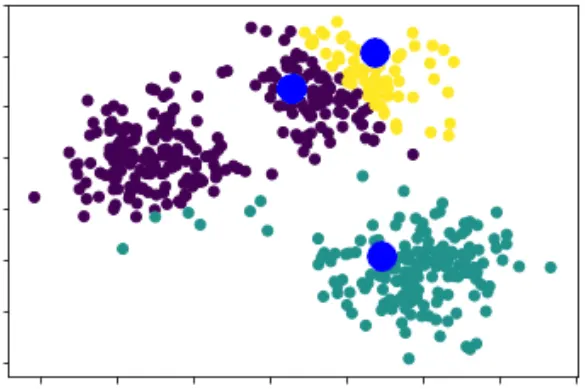
\includegraphics[width=0.6\linewidth]{imagens/1_tEKlqzqtKI3-I0pYSS7oHA.png}
    \caption{Primeira iteração, posição randômica dos centroides \cite{medium_cwi_kmeans}.
}
    \label{fig:centroiderandomico}
\end{figure}
\end{frame}
\subsection{Como Ocorre}
\begin{frame}
    \frametitle{Processo Iterativo e Convergência}
    O algoritmo repete dois passos até que a atribuição dos cluster não mude:
    
    \begin{enumerate}
        \item \textbf{Passo de Atribuição:} Cada ponto é atribuído ao centroide mais próximo.
        \[C_i^{(t)} = \{ \mathbf{x} : ||\mathbf{x} - \boldsymbol{\mu}_i^{(t)}||^2 \le ||\mathbf{x} - \boldsymbol{\mu}_j^{(t)}||^2 \quad \forall j, 1 \le j \le K \}\]
        
        \item \textbf{Passo de Atualização:} Os centroides são recalculados como a média de todos os pontos atribuídos a eles.
        \[\boldsymbol{\mu}_i^{(t+1)} = \frac{1}{|C_i^{(t)}|} \sum_{\mathbf{x} \in C_i^{(t)}} \mathbf{x}\]
    \end{enumerate}
    

\end{frame}
\subsection{Problema Inerentes}
\begin{frame}
    \frametitle{Problemas Inerentes e Soluções}
    \begin{itemize}
        \item \textbf{Sensibilidade à Inicialização:} A escolha aleatória dos centroides iniciais pode levar a resultados ruins.
        \begin{itemize}
            \item \textbf{Solução:} \textbf{K-Means++}, que escolhe os centroides iniciais de forma a estarem distantes uns dos outros.
        \end{itemize}

    \end{itemize}

    \begin{equation}
    P(x) = \frac{D(x)^2}{\sum_{x \in X} D(x)^2},
\end{equation}   
\begin{align*}
    P(x) &= \text{Probabilidade do ponto x ser escolhido como próxima centroide} \\
    D(x)^2 &= \text{Distância para o centróide mais próximo} \\
    \sum_{x \in X} &= \text{Soma de ${D(x)^2}$ para todos os pontos no dataset.}
\end{align*}
\end{frame}
\begin{frame}{Primeiro Centróide}
    \begin{figure}
        \centering
        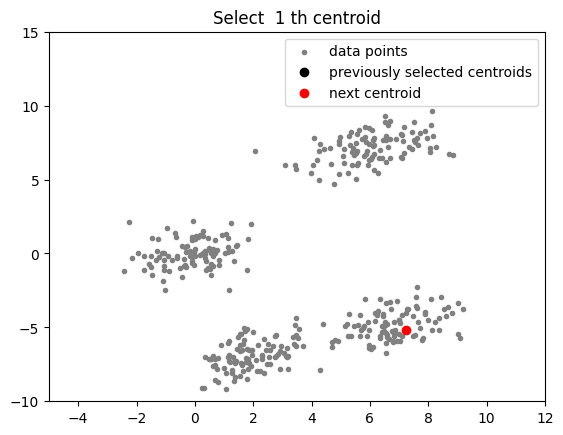
\includegraphics[width=0.7\linewidth]{imagens/kmeans_1.png}
        \caption{Primeiro centroide escolhido\cite{geeksforgeeks_kmeans}.}
        \label{fig:centroide1}
    \end{figure}
\end{frame}
\begin{frame}{Segundo Centróide}
    \begin{figure}
        \centering
        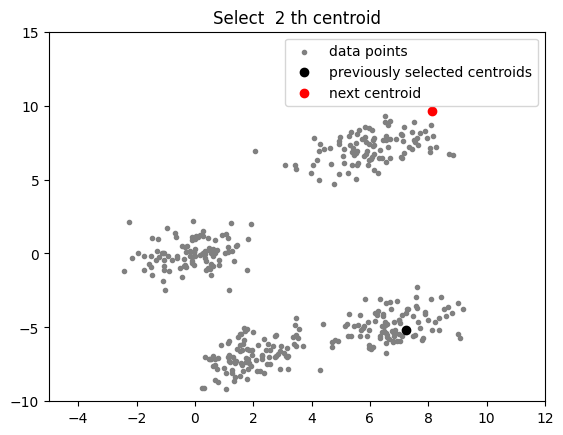
\includegraphics[width=0.7\linewidth]{imagens/kmeans_2.png}
        \caption{Segundo centroide escolhido \cite{geeksforgeeks_kmeans}.}
        \label{fig:centroide2}
    \end{figure}
\end{frame}
\begin{frame}{Terceiro Centróide}
    \begin{figure}
        \centering
        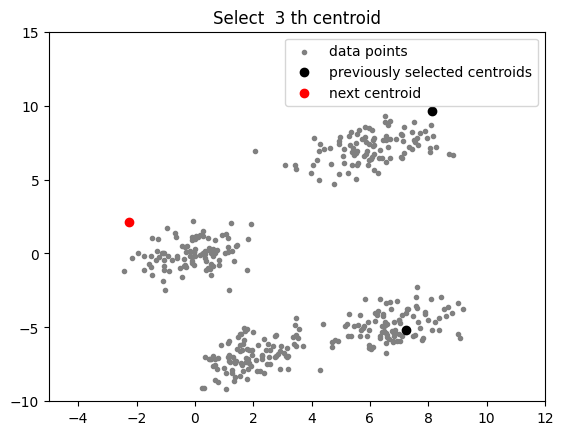
\includegraphics[width=0.7\linewidth]{imagens/kmeans_3.png}
        \caption{Terceiro centroide escolhido\cite{geeksforgeeks_kmeans}.}
        \label{fig:centroide3}
    \end{figure}
\end{frame}
\begin{frame}{Quarto Centróide}
    \begin{figure}
        \centering
        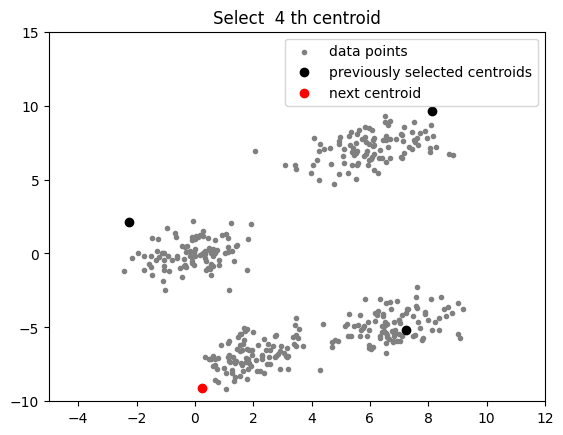
\includegraphics[width=0.7\linewidth]{imagens/kmeans_4.png}
        \caption{Quarto centroide selecionado\cite{geeksforgeeks_kmeans}.}
        \label{fig:centroide4}
    \end{figure}
\end{frame}
\subsection{Métodos e Comparações}
\begin{frame}{Quantidade de Clusters}
   \centering \large{Mas, como podemos determinar a quantidade de cluster?}
   \pause
   \vspace{1cm}
   \begin{itemize}
       \item Método do Cotovelo (\textit{Elbow Method})
       \item Análise da Silhueta  (\textit{Silhouette Analysis})
   \end{itemize}
\end{frame}
\begin{frame}
    \frametitle{Método do Cotovelo (\textit{Elbow Method})}
\begin{figure}
    \centering
    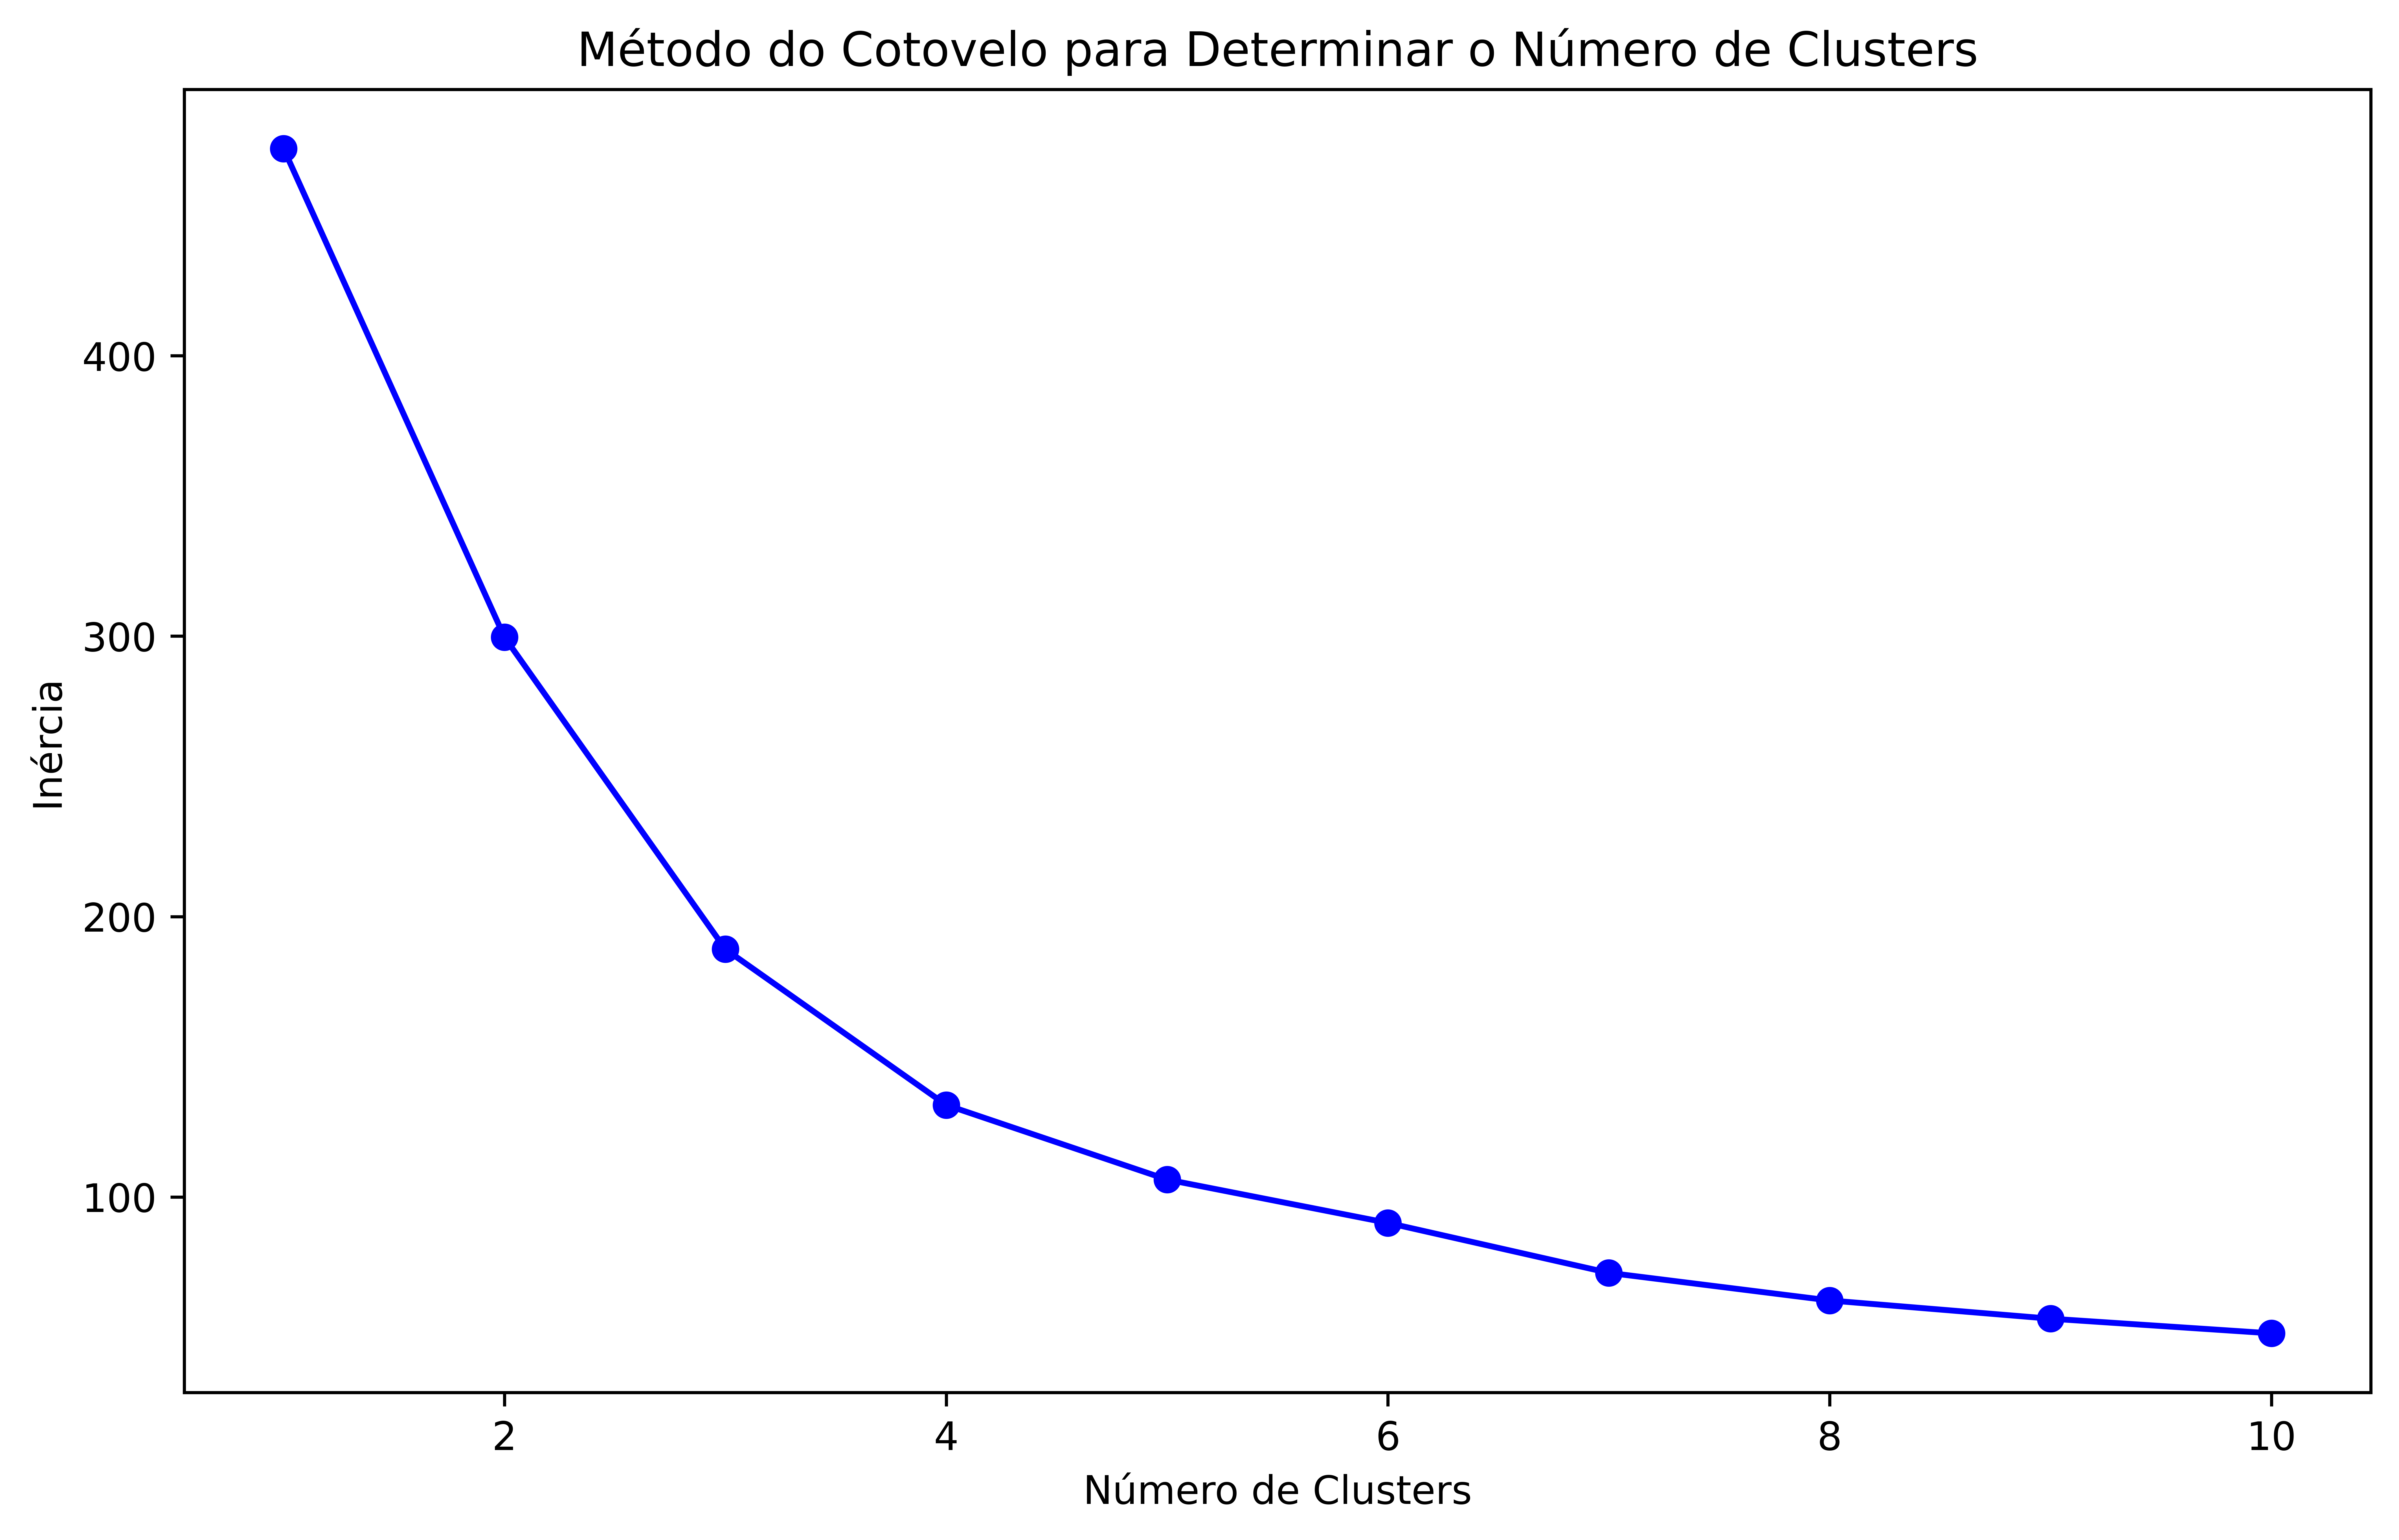
\includegraphics[width=0.85\linewidth]{imagens/metodo_cotovelo.png}
        \label{fig:metododocotovelo}
\end{figure}
\end{frame}

\begin{frame}{Análise da Silhueta  (\textit{Silhouette Analysis})}
    \begin{figure}
    \centering
    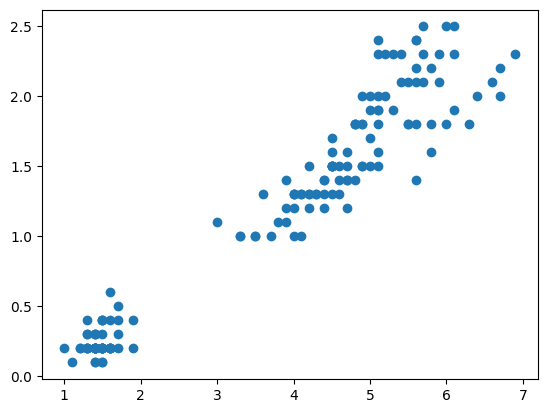
\includegraphics[width=0.6\linewidth]{imagens/output.png}
    \caption{Pontos iniciais.}
    \label{fig:semcluster}
\end{figure}
\end{frame}
\begin{frame}{\(K=5\)}
    \begin{figure}
    \centering
    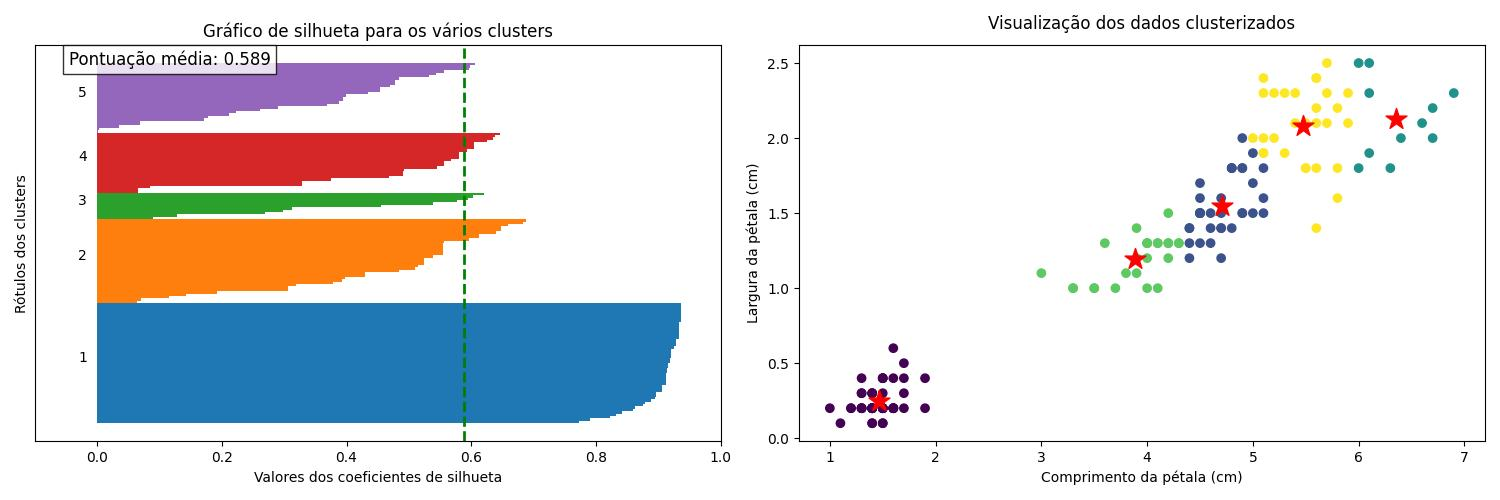
\includegraphics[width=1\linewidth]{imagens/Silhouette_analysis_5.jpg}
    \caption{Pontuação média para cinco cluster.}
    \label{fig:silueta5}
\end{figure}
\end{frame}
\begin{frame}{\(K=4\)}
    \begin{figure}
    \centering
    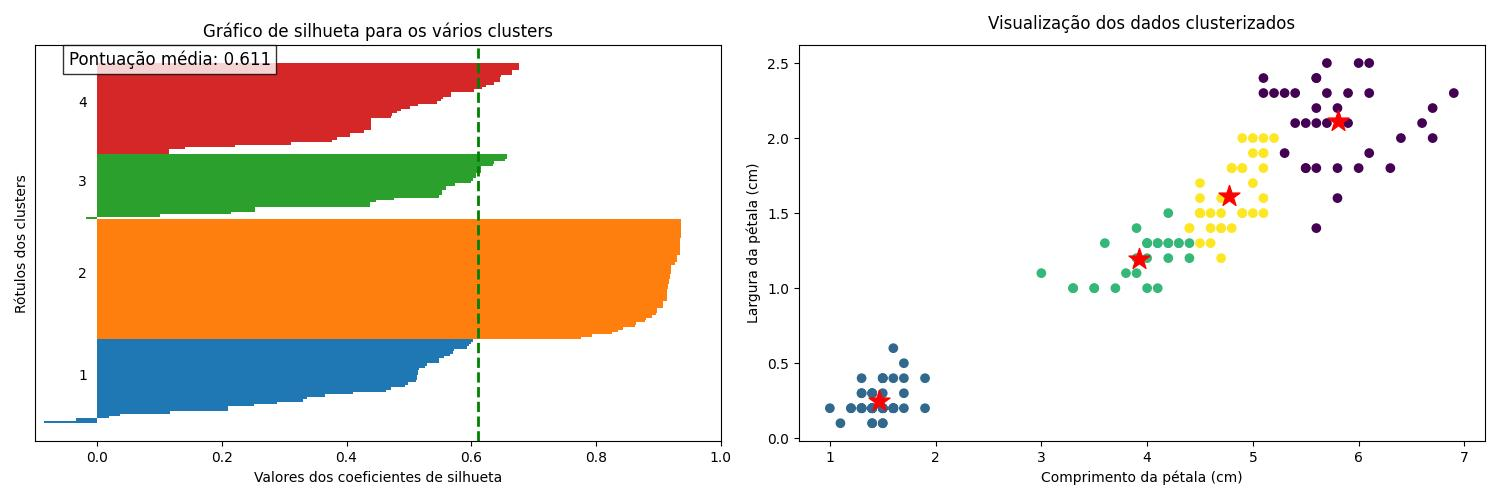
\includegraphics[width=1\linewidth]{imagens/Silhouette_analysis_4.jpg}
    \caption{Pontuação média para quatro cluster.}
    \label{fig:silueta4}
\end{figure}
\end{frame}
\begin{frame}{\(K=3\)}
    \begin{figure}
    \centering
    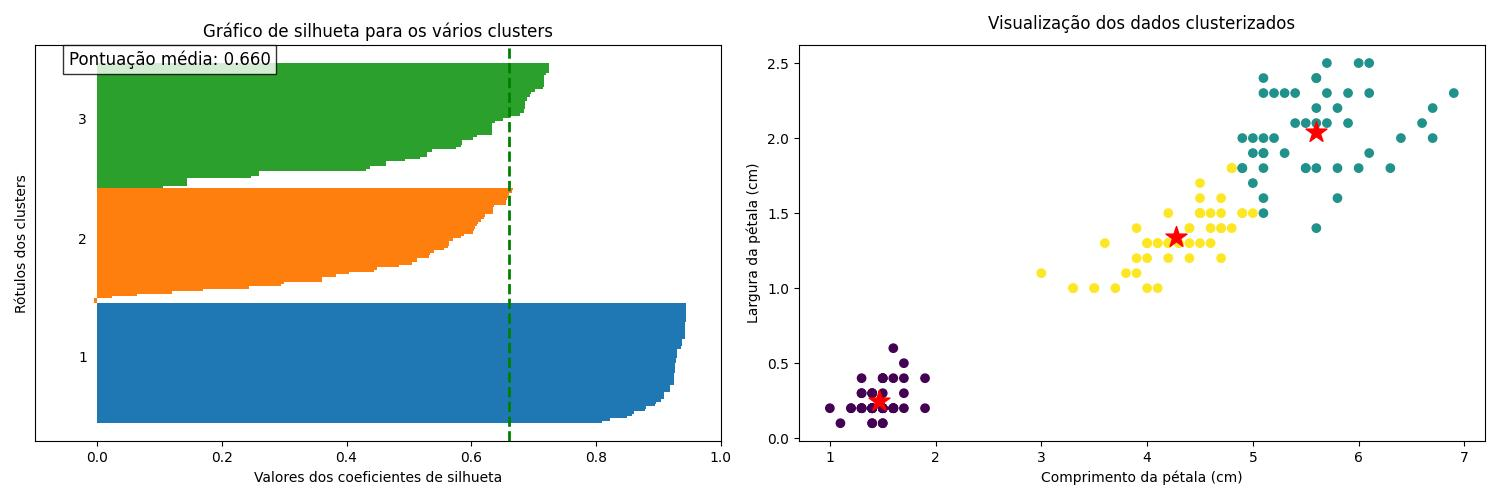
\includegraphics[width=1\linewidth]{imagens/Silhouette_analysis_3.jpg}
    \caption{Pontuação média para três cluster.}
    \label{fig:silueta3}
\end{figure}
\end{frame}
\begin{frame}{\(K=2\)}
    \begin{figure}
    \centering
    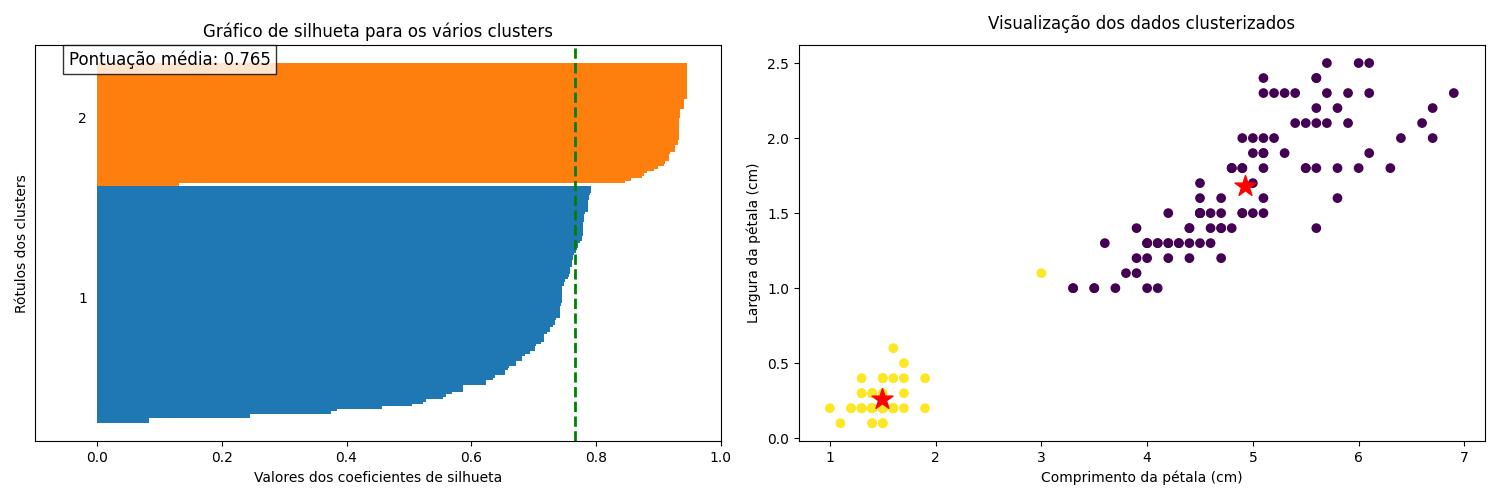
\includegraphics[width=1\linewidth]{imagens/Silhouette_analysis_2.jpg}
    \caption{Pontuação média para dois cluster.}
    \label{fig:silueta2}
\end{figure}
\end{frame}



\begin{frame}{Comparação com Outros Métodos}
    
\begin{table}[h]
\centering


\begin{tabular}{|>{\centering\arraybackslash}m{0.45\textwidth}|>{\centering\arraybackslash}p{0.45\linewidth}|}
\hline
\textbf{K-Means} & \textbf{DBSCAN (Baseado em Densidade)} \\ \hline Requer $K$ pré-definido.& Não requer $K$. \\ \hline
Assume clusters esféricos. & Encontra clusters de formas arbitrárias. \\ \hline
Particiona todos os pontos. & Robusto a outliers (classifica-os como ruído). \\ \hline
Rápido em dados de baixa dimensão. & Não atribui todos os pontos. \\ \hline
\end{tabular}
\caption{Comparação entre entre técnicas, mostrando suas diferenças.}
\label{tab:comparacaokmeans}
\end{table}
\end{frame}
\subsection{Resumo}
\begin{frame}{Resumo Final do K-Means}
    
    \begin{block}{Pontos Fortes}
        \begin{itemize}
            \item \textbf{Simplicidade e Rapidez:} Fácil de implementar e computacionalmente eficiente.
            \item \textbf{Escalabilidade:} Funciona bem em datasets grandes.
        \end{itemize}
    \end{block}
    
    \begin{block}{Pontos Fracos}
        \begin{itemize}
        \item \textbf{Fraquezas:} Vulnerável à inicialização e a outliers. Inadequado para clusters não-esféricos.
    \end{itemize}
    \end{block}
\end{frame}

%%%%%%%%%%%%%%%%%%%%%%%%%%%%%%%%%%%%%%%%%%%%%%%%%%%%%%%%%%%%%%%%%
\section{Estudo de Caso}
\begin{frame}{Introdução ao Estudo de Caso}
    Imagine que somos um banco e precisamos entender o comportamento dos nossos clientes. Como o K-Means e o KNN podem nos ajudar a segmentá-los para um marketing mais eficiente?
\end{frame}

\begin{frame}
    \frametitle{Introdução: K-Means vs. KNN em Finanças}
\begin{itemize}
        \item \textbf{K-Means}: Algoritmo de clusterização não supervisionada que agrupa dados por similaridade, sem necessidade de rótulos prévios.
        \item \textbf{KNN}: Método de classificação supervisionada que faz previsões com base nos \( K \) vizinhos mais próximos, utilizando métricas de distância.
        \item \textbf{Relevância}: Ambos são amplamente utilizados em finanças para segmentação de clientes, previsão de comportamentos e gestão de riscos.
    \end{itemize}
\end{frame}

\begin{frame}
    \frametitle{K-Means: Aplicações Práticas em Finanças}
    \begin{itemize}
        \item \textbf{Segmentação de Clientes}: Agrupar clientes por comportamento para marketing direcionado.
        \item \textbf{Gestão de Risco}: Classificar candidatos a empréstimo por perfil de risco.
        \item \textbf{Detecção de Fraude}: Identificar transações anômalas como outliers.
        \item \textbf{Otimização de Caixas Eletrônicos}: Posicionar recursos em áreas de alta demanda com base em padrões de uso.
    \end{itemize}
\end{frame}

\begin{frame}
    \frametitle{Cenário Hipotético com K-Means: Segmentação de Clientes}
    \textbf{Desafio:} Otimizar o serviço bancário para diferentes perfis de cliente.
\begin{itemize}
        \item \textbf{Passo 1}: Coletar dados demográficos e de transações (e.g., idade, renda anual, gastos mensais) de milhões de contas.
        \item \textbf{Passo 2}: Normalizar os dados para mitigar o impacto de outliers e escalas diferentes.
        \item \textbf{Passo 3}: Aplicar o método do cotovelo para determinar o número ideal de clusters (\( K = 5 \)).
        \item \textbf{Passo 4}: Executar o K-Means para agrupar clientes em perfis, como ``investidores jovens'' e ``poupadores aposentados''.
        \item \textbf{Passo 5}: Desenvolver produtos específicos, como robôs-consultores para jovens e planos de previdência para idosos.
    \end{itemize}
    \textbf{Resultado:} Melhoria na retenção de clientes por meio de estratégias personalizadas.
\end{frame}

\begin{frame}
    \frametitle{Resultados do K-Means: Método do Cotovelo}
    \begin{figure}
        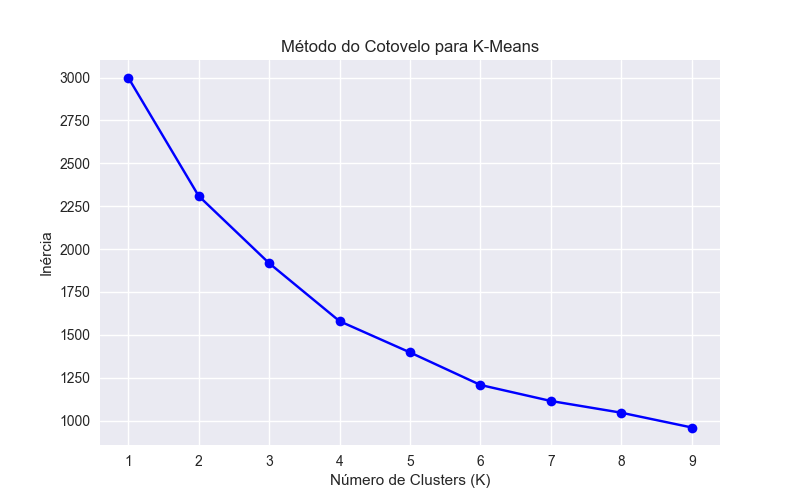
\includegraphics[width=0.8\textwidth]{imagens/elbow_method.png}
        \caption{Método do cotovelo para determinar o número ideal de clusters \( K = 5 \).}
    \end{figure}

\end{frame}

\begin{frame}
    \frametitle{Resultados do K-Means: Segmentação de Clientes}
    \begin{figure}
        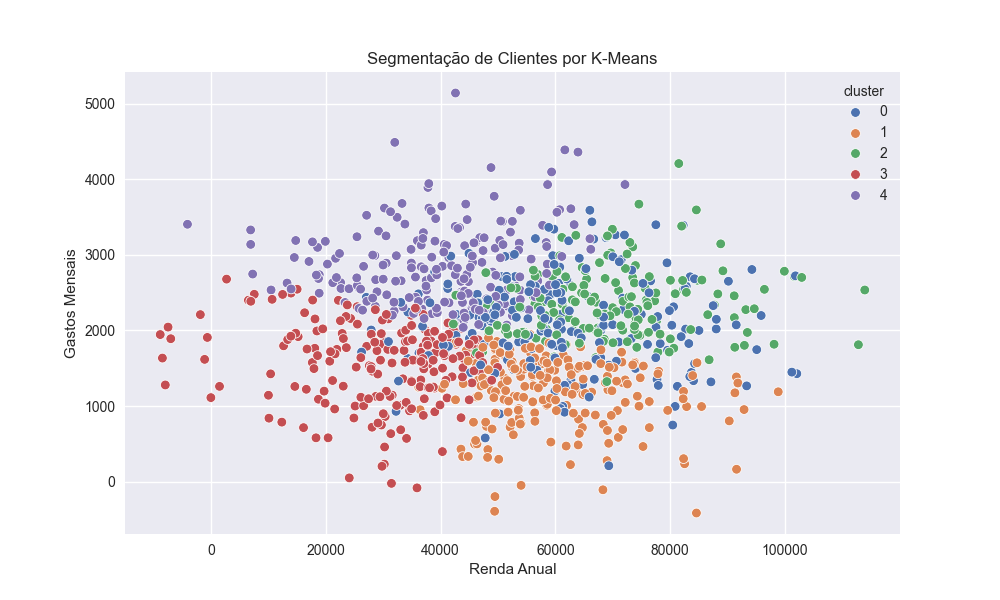
\includegraphics[width=0.8\textwidth]{imagens/customer_segmentation.png}
        \caption{Segmentação de 1000 clientes com base em renda anual e gastos mensais.}
    \end{figure}
 %   \begin{itemize}
%\item Dados sintéticos com 1000 clientes foram agrupados em 5 clusters distintos, refletindo diferentes padrões de comportamento financeiro.
 %       \item A visualização destaca a separação clara entre grupos, permitindo estratégias de marketing direcionadas, como oferta de produtos específicos.
  %  \end{itemize}
\end{frame}

\begin{frame}
    \frametitle{KNN: Aplicações Práticas em Finanças}
    \begin{itemize}
        \item \textbf{Previsão de Ações}: Prever preços de ativos usando similaridades históricas.
        \item \textbf{Score de Crédito}: Classificar a pontuação de risco de candidatos com base em dados passados.
        \item \textbf{Detecção de Fraude}: Identificar transações atípicas com base em desvios de padrões conhecidos
        \item \textbf{Previsão de Falência}: Avaliar o risco de falha de empresas por comparações históricas.
    \end{itemize}
\end{frame}

\begin{frame}
    \frametitle{Cenário Hipotético com KNN: Previsão de Ações}
    \textbf{Desafio:} Prever a direção do preço de uma ação para o próximo dia.
    \begin{itemize}
        \item \textbf{Passo 1}: Coletar dados históricos de uma ação (preços, volume, indicadores técnicos).
        \item \textbf{Passo 2}: Pré-processar os dados, normalizando as características.
        \item \textbf{Passo 3}: Selecionar \( K = 5 \) e a métrica de distância Euclidiana.
        \item \textbf{Passo 4}: Identificar os \( K \) vizinhos mais próximos com base nas condições atuais do mercado.
        \item \textbf{Passo 5}: Prever o movimento (alta ou queda) com base na maioria dos vizinhos.
    \end{itemize}
    \textbf{Resultado:} Aumento na precisão das decisões de compra e venda.
\end{frame}

\begin{frame}
    \frametitle{Resultados do KNN: Previsão de Movimentos de Ações}
    \begin{figure}
        \centering
        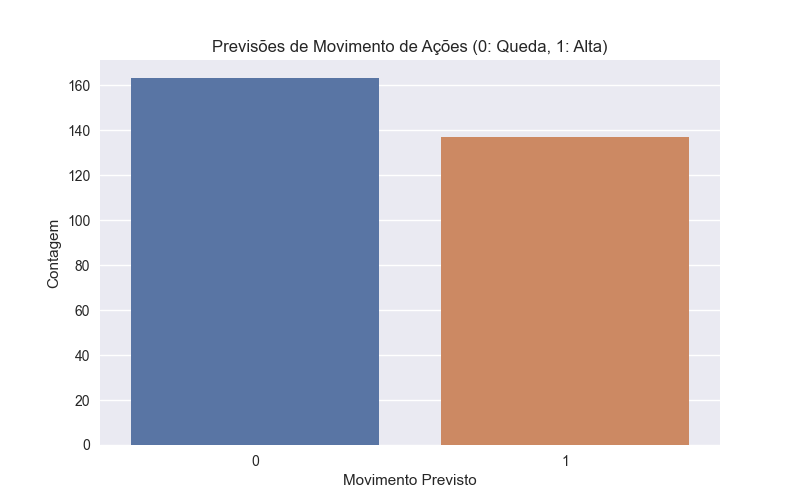
\includegraphics[width=0.6\textwidth]{imagens/stock_prediction.png}
        \caption{Distribuição das previsões de movimento de 300 ações de teste (0: Queda, 1: Alta).}
    \end{figure}

\end{frame}

\begin{frame}
    \frametitle{Insights Comparativos e Futuro}
    \begin{itemize}
        \item \textbf{K-Means}: Eficaz para segmentação não supervisionada, mas requer interpretação humana para nomear clusters e é sensível a inicializações.
        \item \textbf{KNN}: Ideal para previsões supervisionadas, mas computacionalmente intensivo em grandes datasets e sensível à maldição da dimensionalidade.
        \item \textbf{Modelos Híbridos}: A integração de K-Means e KNN pode melhorar a detecção de fraudes ou previsões ao combinar segmentação e classificação.
        \item \textbf{Desafios}: Mitigar ruídos nos dados, reduzir viés e garantir escalabilidade em grandes volumes de dados financeiros.
    \end{itemize}
\end{frame}
%%%%%%%%%%%%%%%%%%%%%%%%%%%%%%%%%%%%%%%%%%%%%%%%%%%%%%%%%%%%%%%%%
\section{Conclusão Final}
%%%%%%%%%%%%%%%%%%%%%%%%%%%%%%%%%%%%%%%%%%%%%%%%%%%%%%%%%%%%%%%%%

\begin{frame}
    \frametitle{Resumo da Apresentação}
    \begin{itemize}
        \item Exploramos a simplicidade e as complexidades dos algoritmos KNN (supervisionado) e K-Means (não supervisionado).
        \item Discutimos a importância das \textbf{métricas de distância}, da \textbf{escolha de K} e do \textbf{pré-processamento} para o sucesso desses modelos.
        \item Demonstramos como, apesar de seus desafios, eles são ferramentas poderosas e versáteis para \textbf{análise e previsão de dados}, com aplicações concretas em finanças e outras áreas.
    \end{itemize}
\end{frame}

\begin{frame}[allowframebreaks]{Referências}
    \bibliographystyle{apalike}
    \bibliography{referencias}
\end{frame}

\begin{frame}
  \begin{center}
    \vfill
    \textbf{\huge Obrigado pela presença de todos!}
    \vspace{1cm}
    \\
     \texttt{brunomendes@fisica.ufmt.br} 
    \vfill
  \end{center}
\end{frame}
\end{document}